\IfFileExists{siamart220329.cls}{%
  \documentclass[review]{siamart220329}
  \newcommand{\usingSIAM}{1}
}{%
  \documentclass[11pt]{article}
  \newcommand{\usingSIAM}{0}
  \usepackage[margin=1in]{geometry}
}

\usepackage[T1]{fontenc}
\usepackage[utf8]{inputenc}
\usepackage{amsmath,amssymb,amsfonts,amsthm,mathtools,bm}
\usepackage{booktabs,tabularx,array}
\newcolumntype{L}[1]{>{\raggedright\arraybackslash}p{#1}}
\newcolumntype{Y}{>{\raggedright\arraybackslash}X}
\usepackage{xcolor}
\usepackage[most]{tcolorbox}
\usepackage{tikz}
\usepackage{pgfplots}
\pgfplotsset{compat=1.18}
\usepackage{enumitem}
\ifnum\usingSIAM=0
\usepackage[hidelinks]{hyperref}
\fi

\emergencystretch=3em
\providecommand{\headers}[2]{}
\makeatletter
\@ifundefined{keywords}{\newenvironment{keywords}{\par\noindent\textbf{Keywords.}\ }{\par}}{}
\@ifundefined{AMS}{\newenvironment{AMS}{\par\noindent\textbf{AMS subject classifications.}\ }{\par}}{}
\makeatother

\newtheorem{theorem}{Theorem}[section]
\newtheorem{proposition}[theorem]{Proposition}
\newtheorem{corollary}[theorem]{Corollary}
\newtheorem{lemma}[theorem]{Lemma}
\newtheorem{assumption}[theorem]{Assumption}
\theoremstyle{definition}
\newtheorem{definition}[theorem]{Definition}
\newtheorem{example}[theorem]{Example}
\theoremstyle{remark}
\newtheorem{remark}[theorem]{Remark}

\newcommand{\R}{\mathbb{R}}
\newcommand{\C}{\mathbb{C}}
\newcommand{\I}{I}
\newcommand{\calX}{\mathcal{X}}
\newcommand{\calY}{\mathcal{Y}}
\newcommand{\calZ}{\mathcal{Z}}
\newcommand{\calU}{\mathcal{U}}
\newcommand{\calV}{\mathcal{V}}
\newcommand{\calA}{\mathcal{A}}
\newcommand{\calE}{\mathcal{E}}
\newcommand{\Sh}{\mathsf{Sh}}
\newcommand{\rank}{\operatorname{rank}}
\newcommand{\range}{\operatorname{range}}
\newcommand{\diag}{\operatorname{diag}}
\newcommand{\dist}{\operatorname{dist}}
\newcommand{\spec}{\operatorname{spec}}
\newcommand{\smin}{\sigma_{\min}}
\newcommand{\smax}{\sigma_{\max}}
\newcommand{\gap}{\operatorname{gap}}
\newcommand{\norm}[1]{\left\lVert #1\right\rVert}
\newcommand{\ip}[2]{\left\langle #1,#2\right\rangle}
\newcommand{\dd}{\,\mathrm{d}}
\newcommand{\pinv}{\dagger}
\newcommand{\eps}{\varepsilon}
\newcommand{\argmin}{\operatorname*{arg\,min}}

\definecolor{siamboxback}{RGB}{248,250,253}
\definecolor{siamboxframe}{RGB}{48,82,118}
\definecolor{siamboxstripe}{RGB}{234,241,249}
\newtcolorbox{siambox}[2][]{%
  enhanced,breakable,colback=siamboxback,colframe=siamboxframe,
  coltitle=black,fonttitle=\bfseries,title={#2},
  boxed title style={colback=siamboxstripe,colframe=siamboxframe,boxrule=0.5pt},
  attach boxed title to top left={xshift=1.2em,yshift=-2mm},
  top=2.5mm,bottom=2.5mm,left=3mm,right=3mm,boxrule=0.6pt,arc=1.2mm,
  before skip=1em,after skip=1em,#1}

\title{A Channel-Conditioned Perturbation Theorem for Hidden Schur-Complement Resolvents}
\author{Anonymous Author}
\date{}
\headers{Channel Condition Numbers}{Anonymous Author}

\begin{document}
\maketitle

\begin{abstract}
Scalar resolvent gain can miss whether a hidden inverse channel is stable,
actuator-accessible, and sensor-visible. We study the restricted transported
inverse channel as a physical map on its singular input subspace. The main
theorem bounds perturbations of this restricted map by a Wedin channel condition
number combining inverse action and singular-subspace separation; a
finite-dimensional lower-bound construction shows the leading scaling is sharp
up to constants. Classical perturbation theory controls the rotation of singular
subspaces, whereas this paper bounds the inverse operator transported by those
subspaces. A local normal form and independent-variation theorem show that
scalar gain, channel conditioning, access, and visibility are distinct
invariants. A composite-map impossibility theorem and fixed-frequency
robust-control corollary show that input-output data do not certify hidden
channel robustness. A nonnormal Schur-complement benchmark then computes the
theorem's quantities directly, while an Orr--Sommerfeld/Squire stress test
illustrates portability to a classical nonnormal PDE discretization.
\end{abstract}

\begin{keywords}
singular vectors, singular subspaces, hidden resolvent, Schur complement, Grassmannian geometry, perturbation theory, Davis--Kahan theorem, Wedin theorem, principal angles, channel condition number, experimental design
\end{keywords}

\begin{AMS}
15A18, 15A42, 47A10, 47A55, 58C40, 65F35, 93B35
\end{AMS}

\section{Introduction}

A scalar inverse norm is an incomplete diagnosis of hidden amplification. If a hidden response equation has the form
\begin{equation}
    \Sh(\theta)\delta z=r,
    \qquad \delta z=\Sh(\theta)^{-1}r,
    \label{eq:hidden-response}
\end{equation}
then $\norm{\Sh^{-1}}_2$ describes only the largest possible amplification. It does not say whether the amplifying residual can be generated by the available controls, whether the hidden displacement can be measured, or whether the relevant singular direction is stable under perturbation. Those questions concern clustered singular subspaces and their stability under metric and parameter variations.

The model is formulated in a coordinate-free setting to capture finite-dimensional generalized singular-value pencils, weighted energy formulations, and compact-resolvent limits of PDE discretizations. Let $\calU$ and $\calV$ be complex Hilbert spaces equipped with their declared inner products. Let $\Sh:\calV\to\calU$ be a bounded linear operator with bounded inverse $R=\Sh^{-1}:\calU\to\calV$. We assume either finite dimensionality or that $R$ is compact, so the nonzero singular values have isolated finite-multiplicity clusters.

A local system $F(x,z;\theta)=0$ linearized at a nominal state yields a hidden Schur complement $\Sh(\theta)$. In finite dimensions this includes the fixed-point representation $z=G(x,z;\theta)+b$ with $\Sh(\theta)=I-D_zG(\theta)$. Externally imposed residuals and observations are represented by bounded linear maps
\begin{equation}
    r=M(\theta)q,
    \qquad y=T(\theta)\delta z,
    \qquad K(\theta)=T(\theta)\Sh(\theta)^{-1}M(\theta).
    \label{eq:composite-response}
\end{equation}
The object of model-based diagnosis is the singular geometry of $\Sh$. The object directly seen in input-output data is the composite map $K$. These are not the same object.

The paper is organized around one central operator: the channel condition number. For a separated cluster, it couples the inverse map carried by the cluster to the separation denominator that controls the left and right singular subspaces. It is not a Davis--Kahan angle in different notation. Davis--Kahan and Wedin estimate how subspaces rotate; the channel condition number estimates how sensitive the operational inverse channel is after that rotation is attached to the resolvent action itself. 

A separate finite-dimensional theorem shows that bounded scalar gain is compatible with unbounded channel conditioning, establishing that the proposed condition number is an independent axis of fragility rather than a repackaging of the resolvent norm.

The theory also includes a matching finite-dimensional lower-bound construction and an input-output impossibility corollary, so the channel condition number is not only useful but structurally unavoidable.

To prevent these interconnected diagnostics from appearing as a loosely related
collection, the manuscript follows a strict logical hierarchy:
\begin{enumerate}
    \item \textbf{Fundamental limits (Section~3):} establishes the core
    restricted-inverse perturbation bound and provides an explicit block-matrix
    construction proving its algebraic sharpness.
    \item \textbf{Structural independence (Section~4):} introduces a canonical
    normal form to prove that the invariants governing this bound---scalar gain,
    Wedin separation, access, and visibility---can vary independently.
    \item \textbf{Diagnostic impossibility (Sections~5--6):} elevates this
    structural independence into a minimax impossibility theorem showing that
    composite input-output data cannot certify internal channel stability.
    \item \textbf{Validation and portability (Sections~7--8):} evaluates the
    hierarchy in a finite-dimensional control benchmark and a nonnormal PDE
    stress test.
\end{enumerate}
The channel condition number $\kappa_J^{\rm chan}$ couples inverse amplification and singular-subspace separation and is the central object of the paper.

The primary objects are the restricted inverse channel $G_J=P_{V,J}\Sh^{-1}P_{U,J}|_{\calU_J}$, the channel condition number $\kappa_J^{\rm chan}$, and access/visibility factors through $M$ and $T$. Threshold margins, metric sensitivity, and design conditions are secondary feasibility constraints that dictate when the primary quantities can be interpreted physically.

\paragraph{Relation to classical perturbation theory.}
Isolated-vector variation may be analyzed by the Hermitian dilation of $\Sh$; clustered variation may be analyzed by Davis--Kahan estimates for the normal equations or, more sharply, by Wedin's singular-subspace theorem \cite{DavisKahan1970,Wedin1972,StewartSun1990,Kato1995}. The present contribution begins after that classical step. It is an explicit algebraic synthesis of Wedin's theorem and the resolvent identity. 

While the derivation of the main theorem uses standard components, isolating the quantity $\kappa_J^{\rm chan}$ exposes the precise mechanism by which subspace rotation infects the inverse action. Thus the paper differentiates itself not by replacing classical bounds, but by introducing the channel condition number and controlling the restricted inverse-channel error that subspace rotation alone does not specify. Classical perturbation theory controls singular subspaces; this paper bounds the inverse operator transported by those subspaces.

\begin{siambox}{Scope, nonclaims, and standing conventions}
Unless otherwise specified, results are stated for boundedly invertible operators $\Sh:\calV\to\calU$ between Hilbert spaces, restricted to isolated finite-multiplicity singular clusters. Cluster projectors are finite-rank Riesz projectors associated with isolated nonzero singular values of the compact inverse; no assertion is made for embedded essential spectrum, continuous spectrum, or non-isolated singular values. Extending these bounds to continuous spectra requires entirely different functional-analytic machinery beyond the scope of this perturbation framework. In finite dimensions this reduces to the usual matrix SVD; in compact-resolvent settings the same statements apply to the corresponding compact inverse or to finite-dimensional Galerkin discretizations. Recent resolvent-analysis guides emphasize that such computations depend materially on the chosen energy norm, discretized operator, and singular-vector implementation \cite{RolandiRibeiroYehTaira2024}. The paper uses Wedin-type singular-subspace perturbation directly in its main theorem; secondary projector estimates remain classical consequences of Hermitian spectral perturbation and Weyl localization \cite{DavisKahan1970,StewartSun1990}. The primary contribution is the channel condition number and its strict restricted inverse-channel bound containing explicit second-order cross terms.

These objects are not supplied by scalar resolvent-gain analyses and are not interchangeable with ordinary subspace-angle estimates. Singular values, angles, and projectors are physically meaningful only after the residual and hidden inner products have been declared.
\end{siambox}

\paragraph{Notation.}
The symbol $*$ denotes transpose in the real case and conjugate transpose in the complex case. All operator norms are spectral norms unless explicitly marked by a Frobenius subscript. Principal angles and projectors are computed in the inner product declared for the corresponding space.

\section{Singular channels, weights, and invariant primitives}\label{sec:primitives}

For a finite-dimensional problem, or for an isolated finite-multiplicity singular cluster of a compact inverse, write
\begin{equation}
    \Sh v_i=\sigma_i u_i,
    \qquad
    \Sh^*u_i=\sigma_i v_i,
    \qquad
    0<\sigma_1\leq\sigma_2\leq\cdots,
    \label{eq:svd}
\end{equation}
with orthonormal left and right singular vectors in the declared Hilbert metrics. For the inverse problem,
\begin{equation}
    \Sh^{-1}u_i=\sigma_i^{-1}v_i.
    \label{eq:inverse-action}
\end{equation}
Thus $u_i$ is the exciting residual direction and $v_i$ is the hidden displacement direction.

Physical coordinates often carry non-Euclidean metrics. If the residual and hidden norms are governed by positive definite weights $W_r,W_z$, the metric singular analysis of the inverse map $R=\Sh^{-1}:r\mapsto z$ is the Euclidean singular analysis of the whitened operator
\begin{equation}
    \widehat R=W_z^{1/2}\Sh^{-1}W_r^{-1/2}.
    \label{eq:weighted-resolvent}
\end{equation}
The notation preserves the inverse-map interpretation: a right singular vector $\widehat u_i$ of $\widehat R$ is a whitened residual direction and a left singular vector $\widehat v_i$ is a whitened hidden direction, $\widehat R\widehat u_i=\mu_i\widehat v_i$. The corresponding physical directions are
\begin{equation}
    u_i^{(W)}=W_r^{-1/2}\widehat u_i,
    \qquad
    v_i^{(W)}=W_z^{-1/2}\widehat v_i,
    \qquad
    \mu_i=\norm{R u_i^{(W)}}_{W_z}/\norm{u_i^{(W)}}_{W_r}.
    \label{eq:weighted-physical-vectors}
\end{equation}
These directions are orthonormal in the weighted inner products. The Euclidean SVD of $\Sh$ and the weighted SVD of the inverse map are different diagnostic objects unless the metrics and conventions have been explicitly matched.

\begin{definition}[access and visibility]
For an isolated channel, the access and visibility seminorms are $a_i=\norm{u_i^*M}_2$ and $b_i=\norm{Tv_i}_2$. The measured contribution of the channel is exactly
\begin{equation}
    K_i=\sigma_i^{-1}(Tv_i)(u_i^*M).
    \label{eq:rank-one-contribution}
\end{equation}
For an $r$-dimensional cluster $J$, the rank-sensitive quantities are
\begin{equation}
    A_J=U_J^*M,
    \qquad B_J=TV_J,
    \qquad \rank A_J,
    \qquad \rank B_J,
    \label{eq:cluster-access-visibility}
\end{equation}
where $U_J=[u_j]_{j\in J}$ and $V_J=[v_j]_{j\in J}$.
\end{definition}

For a cluster $J$, let $\calU_J=\range(U_J)$ and $\calV_J=\range(V_J)$, with corresponding projectors $P_{U,J}$ and $P_{V,J}$.

\begin{definition}[clustered singular channel]
The ambient representative of the clustered inverse channel is
\begin{equation}
    \mathcal G_J=P_{V,J}\Sh^{-1}P_{U,J}:\calU\to\calV .
\end{equation}
The physical restricted channel associated with $J$ is the coordinate-free map
\begin{equation}
    G_J=\mathcal G_J|_{\calU_J}:\calU_J\to\calV .
    \label{eq:restricted-inverse}
\end{equation}
In singular-vector coordinates, $[G_J]_{V,U}=\diag(\sigma_j^{-1}:j\in J)$.
\end{definition}


\section{Main theorem: Hilbert-Space Restricted Inverse Perturbation Bound}\label{sec:perturbation}

This section contains the core restricted inverse-channel bound. It is stated between Hilbert spaces so that generalized singular-value pencils, weighted energy metrics, and compact-resolvent PDE limits are included in the notation rather than appended as separate cases. The proof remains an algebraic synthesis of Wedin singular-subspace perturbation and the resolvent identity.

Let $\calU$ and $\calV$ be Hilbert spaces with inner products $\ip{\cdot}{\cdot}_{\calU}$ and $\ip{\cdot}{\cdot}_{\calV}$. Let $\Sh:\calV\to\calU$ be boundedly invertible and let $R=\Sh^{-1}:\calU\to\calV$. In infinite dimensions assume $R$ is compact, or restrict attention to an isolated finite-multiplicity singular cluster. Let $\widetilde\Sh=\Sh+E$, with $E:\calV\to\calU$ bounded, and let $\widetilde R=\widetilde\Sh^{-1}$. For a separated singular cluster $J$, define the Wedin separation
\begin{equation}
    \omega_J=\min_{j\in J,\;k\notin J}|\sigma_j-\sigma_k|>0.
    \label{eq:wedin-gap}
\end{equation}
The perturbed cluster $\widetilde J$ is selected by the standard spectral matching for isolated singular clusters. Under $\norm{E}_{\calV\to\calU}<\omega_J/2$, the matched cluster preserves its dimension.

\begin{definition}[Wedin channel condition number]
\label{def:channel-condition-number}
Let $P_{U,J}$ and $P_{V,J}$ be the orthogonal Riesz projectors onto the left and right singular subspaces in the declared Hilbert metrics of $\calU$ and $\calV$. For the ambient representative $\mathcal G_J=P_{V,J}RP_{U,J}:\calU\to\calV$, define
\begin{equation}
    \kappa_J^{\rm chan}
    =\frac{\norm{\mathcal G_J}_{\calU\to\calV}}{\omega_J}.
    \label{eq:channel-condition-number}
\end{equation}
\end{definition}

\begin{definition}[projection-induced restricted-map error]
\label{def:restricted-map-error}
Let $G_J=P_{V,J}RP_{U,J}|_{\calU_J}:\calU_J\to\calV_J$. The physical restricted error is measured on the original residual cluster by
\begin{equation}
    \norm{\widetilde G_J-G_J}_{\calU_J\to\calV}
    :=
    \sup_{u\in\calU_J,\ \norm{u}_{\calU}=1}
    \norm{\widetilde P_{V,J}\widetilde\Sh^{-1}\widetilde P_{U,J}u
    -P_{V,J}\Sh^{-1}P_{U,J}u}_{\calV} .
    \label{eq:restricted-map-error}
\end{equation}
Because this restricted error is bounded above by the ambient operator error $\norm{\widetilde{\mathcal G}_J-\mathcal G_J}_{\calU\to\calV}$, the theorem is proved on the ambient representative without altering the operational metric.
\end{definition}
The error is deliberately measured in the full $\calV$-norm, rather than only inside $\calV_J$, because the physical displacement error includes leakage into the ambient hidden space.


\begin{theorem}[Restricted Inverse Perturbation Bound]
\label{thm:channel-conditioned-stability}
Let $\Sh$ be invertible and let $J$ be a singular cluster with Wedin separation $\omega_J>0$. Put $e=\norm{E}_{\calV\to\calU}$ and assume $e<\omega_J/2$ and $\norm{R}_{\calU\to\calV}e<1$. Let $\widetilde{\mathcal G}_J$ be the perturbed ambient restricted inverse channel selected by Wedin spectral matching. Then the exact restricted-map error satisfies the strict nonasymptotic bound:
\begin{align}
    \max\left\{
    \norm{\widetilde{\mathcal G}_J-\mathcal G_J}_{\calU\to\calV},
    \norm{\widetilde G_J-G_J}_{\calU_J\to\calV}
    \right\}
    &\leq
    \left(\frac{2\norm{R}_{\calU\to\calV}}{\omega_J}+\norm{R}_{\calU\to\calV}^2\right)e
    +C_J(e)\frac{e^2}{\omega_J},
    \label{eq:channel-conditioned-bound-explicit}
\end{align}
where the explicit second-order bounding coefficient is:
\begin{equation}
    C_J(e)=\frac{2\norm{R}_{\calU\to\calV}^2}{1-\norm{R}_{\calU\to\calV}e}
    +\frac{\norm{R}_{\calU\to\calV}}{\omega_J-e}.
    \label{eq:channel-second-order-constant}
\end{equation}
Equivalently, the linear part isolated by the channel condition number is:
\begin{equation}
    \left(
        2\kappa_J^{\rm chan}\frac{\norm{R}_{\calU\to\calV}}{\norm{\mathcal G_J}_{\calU\to\calV}}
        +\norm{R}_{\calU\to\calV}^2
    \right)e.
    \label{eq:channel-conditioned-bound}
\end{equation}
For the most amplified selected cluster, where $\norm{\mathcal G_J}_{\calU\to\calV}=\norm{R}_{\calU\to\calV}$, the first-order sensitivity reduces exactly to $(2\kappa_J^{\rm chan}+\norm{R}_{\calU\to\calV}^2)e$.
\end{theorem}
\begin{remark}[Operator-theoretic limitation]
The Hilbert-space formulation is intentionally restricted to isolated finite-multiplicity singular clusters. In compact-resolvent PDE settings this is the regime captured by Galerkin or collocation discretizations. The theorem is not a statement about embedded essential spectrum, nonclosed ranges, or singular values without a separating Wedin gap.
\end{remark}


\begin{proof}
Use the exact decomposition
\begin{align}
\widetilde P_{V,J}\widetilde R\widetilde P_{U,J}-P_{V,J}RP_{U,J}
&=(\widetilde P_{V,J}-P_{V,J})\widetilde R\widetilde P_{U,J}
  +P_{V,J}(\widetilde R-R)\widetilde P_{U,J}  \notag\\
&\quad +P_{V,J}R(\widetilde P_{U,J}-P_{U,J}).
\label{eq:wedin-channel-decomposition}
\end{align}
The first line of this bound is the leading linear estimate; the remaining terms are explicit higher-order safeguards.
For isolated finite-multiplicity singular clusters, Wedin's direct singular-subspace theorem gives the nonasymptotic estimates
\begin{equation}
    \norm{\widetilde P_{V,J}-P_{V,J}}_{\calV\to\calV}\leq \frac{e}{\omega_J-e},
    \qquad
    \norm{\widetilde P_{U,J}-P_{U,J}}_{\calU\to\calU}\leq \frac{e}{\omega_J-e},
    \label{eq:direct-wedin-projector}
\end{equation}
for the matched cluster. The resolvent identity gives
\begin{equation}
    \norm{\widetilde R-R}_{\calU\to\calV}\leq
    \frac{\norm{R}_{\calU\to\calV}^2e}{1-\norm{R}_{\calU\to\calV}e},
    \qquad \norm{\widetilde R}_{\calU\to\calV}\leq \frac{\norm{R}_{\calU\to\calV}}{1-\norm{R}_{\calU\to\calV}e}.
    \label{eq:resolvent-nonasymptotic}
\end{equation}
Substitution in \eqref{eq:wedin-channel-decomposition} yields the strict bound
\begin{equation}
    \norm{\widetilde{\mathcal G}_J-\mathcal G_J}_{\calU\to\calV}
    \leq
    \frac{e}{\omega_J-e}\frac{\norm{R}_{\calU\to\calV}}{1-\norm{R}_{\calU\to\calV}e}
    +\frac{\norm{R}_{\calU\to\calV}^2e}{1-\norm{R}_{\calU\to\calV}e}
    +\norm{R}_{\calU\to\calV}\frac{e}{\omega_J-e}.
    \label{eq:channel-bound-nonasymptotic}
\end{equation}
For $e<\omega_J/2$ and $\norm{R}_{\calU\to\calV}e<1$, algebraic factorization of the first and third terms splits their linear contribution $2\norm{R}_{\calU\to\calV}e/\omega_J$ from a controlled remainder, while the middle term splits into $\norm{R}_{\calU\to\calV}^2e$ and its resolvent remainder. This yields \eqref{eq:channel-conditioned-bound-explicit} with $C_J(e)$ as in \eqref{eq:channel-second-order-constant}. Since $\norm{\mathcal G_J}_{\calU\to\calV}/\omega_J=\kappa_J^{\rm chan}$, the linear subspace-transport contribution is identically $2\kappa_J^{\rm chan}(\norm{R}_{\calU\to\calV}/\norm{\mathcal G_J}_{\calU\to\calV})e$.
\end{proof}

\subsection{Structural necessity of the bounds}\label{sec:structural-necessity}
The inverse-gain factor and the singular-separation denominator in Theorem~\ref{thm:channel-conditioned-stability} are both structurally unavoidable. The following compact proposition shows that a uniform error bound must contain the bilinear product of inverse gain and separation, verifying that neither factor can be omitted.

\begin{proposition}[Structural necessity of the bilinear gain-gap product]
\label{prop:structural-necessity}
Let $\sigma, \omega > 0$ and consider the hidden resolvent and its perturbation:
\begin{equation}
    \Sh_0 = \begin{bmatrix} \sigma & 0 \\ 0 & \sigma+\omega \end{bmatrix},
    \qquad
    E = \begin{bmatrix} 0 & e \\ e & 0 \end{bmatrix}.
\end{equation}
For the leading channel $J=\{1\}$, the Wedin separation is $\omega_J = \omega$, and the unperturbed restricted inverse map is $\mathcal{G}_J = \sigma^{-1} e_1 e_1^*$. 
As $e \to 0$, the perturbation of the ambient restricted inverse channel satisfies the exact leading-order expansion:
\begin{equation}
    \norm{\widetilde{\mathcal{G}}_J - \mathcal{G}_J}_2 = e \left( \frac{2\sigma+\omega}{\sigma(\sigma+\omega)\omega} \right) + O(e^2).
\end{equation}
In the physically relevant highly amplified regime where $\sigma \ll \omega \ll 1$, this leading-order error is asymptotically equivalent to the channel condition number:
\begin{equation}
    \frac{e}{\sigma \omega} = \kappa_J^{\rm chan} e.
\end{equation}
\end{proposition}

\begin{proof}
The perturbed eigenvalues are the roots of the characteristic polynomial $\lambda^2 - (2\sigma+\omega)\lambda + \sigma(\sigma+\omega)-e^2=0$. A standard Taylor expansion in $e$ shows the perturbed smallest singular value is $\tilde{\sigma} = \sigma - e^2/\omega + O(e^4)$, while the corresponding unnormalized right singular vector shifts as $\tilde{v}_1 = [1, -e/\omega]^T + O(e^2)$. Normalizing the projectors and evaluating $\widetilde{\mathcal{G}}_J = \tilde{\sigma}^{-1} \tilde{v}_1 \tilde{v}_1^*$ against $\mathcal{G}_J$ yields the stated cross-term. The asymptotic collapse to $(\sigma \omega)^{-1}$ is immediate by retaining the highest-order poles.
\end{proof}




\subsection{Sharpness of the leading restricted inverse-channel scaling}\label{sec:near-sharpness}

The preceding bound is a synthesis of subspace perturbation and the resolvent
identity, but the leading dependences are not artifacts of the proof. The next
result records a finite-dimensional lower-bound construction showing that both
the subspace-transport factor and the inverse-resolvent factor are structurally
unavoidable up to absolute constants.

\begin{theorem}[Sharpness of the leading restricted inverse-channel scaling]
\label{thm:near-sharpness-main}
There is a universal constant $c_0>0$ with the following property. For all
sufficiently small $e>0$, there exist finite-dimensional invertible operators
$\Sh$ and perturbations $E$ with $\norm{E}_2=e$ and an isolated one-dimensional
channel $J$ such that
\begin{equation}
    \norm{\widetilde G_J-G_J}_2
    \ge
    c_0\left(
    \frac{\norm{\mathcal G_J}_2\norm{R}_2}{\omega_J}
    +
    \norm{R}_2^2
    \right)e
\end{equation}
whenever the perturbed channel is identified by continuation.
\end{theorem}

\begin{proof}
The lower bound is obtained by a precise direct-sum construction. Define the
$3\times3$ unperturbed operator and structured perturbation
\begin{equation}
    \Sh=
    \begin{bmatrix}
    \sigma & 0 & 0\\
    0 & \sigma & 0\\
    0 & 0 & \sigma+\omega
    \end{bmatrix},
    \qquad
    E=\frac{e}{\sqrt{2}}
    \begin{bmatrix}
    0 & 0 & 1\\
    0 & 1 & 0\\
    1 & 0 & 0
    \end{bmatrix},
\end{equation}
acting on Euclidean $\R^3$. The perturbation satisfies $\norm{E}_2=e$.
Let $J=\{1,2\}$ denote the highly amplified singular cluster, so that
$\norm{R}_2=\sigma^{-1}$ and the separating Wedin gap is
$\omega_J=\omega$.

The perturbation separates two mechanisms. On the $(1,3)$ plane, the
off-diagonal perturbation rotates one component of the amplified cluster toward
the neighboring singular direction. Proposition~\ref{prop:structural-necessity}
therefore gives a restricted-map error bounded below by a universal constant
multiple of
\begin{equation}
    e\,\sigma^{-1}(\sigma+\omega)^{-1}\omega^{-1},
\end{equation}
which, in the separated amplified regime, is bounded below by a universal
constant multiple of
\[
    e\,\frac{\norm{\mathcal G_J}_2\norm{R}_2}{\omega_J}.
\]
On the second amplified coordinate, the diagonal perturbation produces the
scalar resolvent error
\begin{equation}
    \left|(\sigma+e/\sqrt{2})^{-1}-\sigma^{-1}\right|,
\end{equation}
which is bounded below by a universal constant multiple of
\[
    e\,\norm{R}_2^2
\]
for $e\le \sigma/2$.

The restricted error of the direct sum is the maximum of the two block errors.
Since $\max(A,B)\ge (A+B)/2$ for nonnegative $A,B$, the total restricted-map
error satisfies, for sufficiently small $e$,
\begin{equation}
    \norm{\widetilde G_J-G_J}_2
    \ge
    c_0
    \left(
    \frac{\norm{\mathcal G_J}_2\norm{R}_2}{\omega_J}
    +
    \norm{R}_2^2
    \right)e
\end{equation}
for a universal constant $c_0>0$. The construction confirms that neither the
subspace-transport term nor the inverse-resolvent term can be removed from the
leading scaling.
\end{proof}

Thus the main theorem is conservative only in absolute constants and in the
particular second-order envelope. Its dependence on inverse gain, singular
separation, and the resolvent identity is structurally necessary.

\subsection{Canonical normal form and independent variation}\label{sec:decoupling}

Having established the fundamental perturbation bounds, we now show that the
quantities governing those bounds are mathematically irreducible. The restricted
inverse channel is not merely a diagnostic heuristic; it has a strict local
normal form. For an isolated cluster, the system decomposes into
distinct geometric ingredients: inverse gain, singular-subspace separation, and
access/visibility architecture.

\begin{proposition}[Local normal form for a separated hidden channel]
\label{prop:normal-form}
Let $J$ be an isolated singular cluster of $\Sh$. Under the orthogonal direct
sum decompositions $\calU=\calU_J\oplus\calU_J^\perp$ and
$\calV=\calV_J\oplus\calV_J^\perp$, the hidden operator and the experimental
maps partition exactly as the block operators
\begin{equation}
    \Sh =
    \begin{bmatrix}
    \Sigma_J & 0\\
    0 & \Sigma_\perp
    \end{bmatrix},
    \qquad
    M =
    \begin{bmatrix}
    M_J\\
    M_\perp
    \end{bmatrix},
    \qquad
    T =
    \begin{bmatrix}
    T_J & T_\perp
    \end{bmatrix}.
\end{equation}
The measured composite contribution of the channel is strictly
$T_J\Sigma_J^{-1}M_J$. The structural stability and experimental relevance of
this channel are governed by four canonical invariants: the scalar inverse gain
$\norm{\Sigma_J^{-1}}_{\calU\to\calV}$, the Wedin separation
$\min_{\sigma\in\sigma(\Sigma_J),\,\tau\in\sigma(\Sigma_\perp)}|\sigma-\tau|$, the actuator access
$\smin(M_J)$, and the sensor visibility $\smin(T_J)$.
\end{proposition}

\begin{proof}
Let $P_{U,J}$ and $P_{V,J}$ denote the singular-cluster projectors and use the
orthogonal decompositions induced by these projectors. Since $\Sh$ maps
$\calV_J$ to $\calU_J$ and $\calV_J^\perp$ to $\calU_J^\perp$ in the singular
basis, its block representation has no off-diagonal channel terms. The
restrictions of $\Sh$ to the two components are $\Sigma_J$ and $\Sigma_\perp$.
The block decompositions of $M$ and $T$ are obtained by applying the same
orthogonal projectors to their ranges and domains. Restricting $R=\Sh^{-1}$ to
the channel block gives $G_J=\Sigma_J^{-1}$ in this direct-sum representation,
hence the measured channel contribution is $T_J\Sigma_J^{-1}M_J$.
\end{proof}

A fundamental question in robust control and pseudospectral analysis is whether
these local invariants are reducible to scalar gain. The following theorem shows
that they are not.

\begin{theorem}[Independent variation of canonical channel invariants]
\label{thm:complete-separation}
For any prescribed scalar inverse gain $g>1$, channel condition number $c>0$,
access level $a\in(0,1]$, and visibility level $b\in(0,1]$, after choosing the
remaining singular value sufficiently separated from the selected cluster, there
exists a finite-dimensional realization $(\Sh,M,T)$ and a one-dimensional
isolated channel $J$ such that
\begin{equation}
    \norm{\Sh^{-1}}_2=g,\qquad
    \kappa_J^{\rm chan}=c,\qquad
    \smin(U_J^*M)=a,\qquad
    \smin(TV_J)=b.
\end{equation}
\end{theorem}

\begin{proof}
Let $\calU=\calV=\R^3$ equipped with the Euclidean metric. Define the singular
value decomposition $\Sh=U\Sigma V^*$ with fixed orthogonal matrices $U,V$ and
singular values
\begin{equation}
    \Sigma=\operatorname{diag}\left(g^{-1},\,g^{-1}+g/c,\,\rho\right),
    \qquad
    \rho>g^{-1}+g/c+1 .
\end{equation}
The scalar inverse norm is exactly $\norm{\Sh^{-1}}_2=g$, bounding worst-case
amplification independently of $c$. For the leading channel $J=\{1\}$, the
Wedin separation is strictly $\omega_J=g/c$ by construction. Therefore
\begin{equation}
    \kappa_J^{\rm chan}
    =
    \frac{\norm{\mathcal G_J}_2}{\omega_J}
    =
    \frac{g}{g/c}
    =
    c .
\end{equation}
To prescribe access and visibility without changing the hidden singular
geometry, set
\begin{equation}
    M=U
    \begin{bmatrix}
    a\\
    \sqrt{1-a^2}\\
    0
    \end{bmatrix},
    \qquad
    T=
    \begin{bmatrix}
    b & \sqrt{1-b^2} & 0
    \end{bmatrix}V^* .
\end{equation}
Then $\smin(U_J^*M)=a$ and $\smin(TV_J)=b$. Thus scalar gain, channel
conditioning, actuator access, and sensor visibility can be prescribed
independently.
\end{proof}

This theorem makes the paper's thesis mathematically unavoidable. While the
underlying mechanism of singular-value separation is classical, its consequence
for the transported restricted inverse channel is not captured by scalar gain.
Scalar resolvent gain, channel conditioning, actuator access, and sensor
visibility are independent geometric invariants.

\section{Gauge-invariant clustered response}\label{sec:clustered-response}

In singular-vector coordinates the cluster contribution to the measured response is $K_J=TV_J\Sigma_J^{-1}U_J^*M$. This is basis-dependent notation for the coordinate-free map $TG_JM$. If $\widehat U_J=U_JQ_U$ and $\widehat V_J=V_JQ_V$, with $Q_U,Q_V$ unitary, then $[G_J]_{\widehat V,\widehat U}=Q_V^*[G_J]_{V,U}Q_U$. Componentwise interpretation inside a close cluster is therefore spurious without an external convention. The stable clustered quantities are $G_J$, the projectors $P_{U,J}, P_{V,J}$, and the access/visibility matrices.

\section{Diagnostic Feasibility and Geometric Nonidentifiability}\label{sec:thresholds}

The secondary results in this section identify when the primary quantities ($G_J$ and $\kappa_J^{\rm chan}$) may be interpreted physically. They are formulated as feasibility constraints rather than as optimization heuristics.

\subsection{Threshold events and metric sensitivity}

Singular-channel analysis frequently encounters rank events and threshold crossings. For a threshold $\tau>0$, the spectral projector $P_{V,\tau}$ of $\Sh^*\Sh$ associated with $[0,\tau^2]$ is stable only bounded away from collisions. If $\spec(\Sh^*\Sh)\cap(\tau^2-\rho,\tau^2+\rho)=\varnothing$, Weyl localization and the Davis--Kahan theorem guarantee a local Lipschitz bound proportional to $1/\rho$ \cite{DavisKahan1970}. A thresholded channel report without reporting this gap $\rho$ is not reproducible.

Similarly, metric declaration is not a cosmetic convention. If the residual and hidden metrics are perturbed as $\widetilde W_z^{1/2}R\widetilde W_r^{-1/2}$, the whitened operator changes. If the operator error $\delta_W$ is bounded away from the metric spectral gap $\rho_J/2$, the Davis--Kahan estimate bounds the projector rotation. 

\begin{definition}[metric robustness radius]\label{def:metric-robustness-radius}
For a declared weight class $\mathfrak W(s)$ parameterized by $s$, the metric robustness radius $R_{\rm met}(\vartheta)$ is the supremum over $s \ge 0$ such that the localized right singular projector rotates by at most an angle $\vartheta$ from its nominal state. 
\end{definition}
This operationalizes metric uncertainty by reporting how far the weights may move before the channel orientation exceeds a declared physical tolerance.

\subsection{Diagnostic feasibility constraints}

In experimental or robust-control applications, an oracle design aims to excite and observe the hidden cluster. Rather than formulating a highly non-convex optimization problem with arbitrary penalty weights, a physically meaningful robust design point is any configuration that satisfies a strict set of feasibility margins.

\begin{definition}[Channel-Robust Feasibility]
\label{def:channel-robust-feasibility}
Given tolerances $g_{\rm min}, \omega_{\rm min}, w_{\rm max}, a_{\rm min}, b_{\rm min} > 0$, a design configuration parameterized by $(\theta, Q)$ is channel-robust feasible if it satisfies the inverse gain and stability conditions:
\begin{equation}
    \norm{G_J(\theta)}_2\geq g_{\rm min},\qquad
    \omega_J(\theta)\geq\omega_{\rm min},\qquad
    \delta_W(\theta)\leq w_{\rm max},
    \label{eq:channel-design-gain-access}
\end{equation}
and strict bounds on access and visibility:
\begin{equation}
    \smin(U_J(\theta)^*M(\theta)Q)\geq a_{\rm min}>0,
    \qquad
    \smin(T(\theta)V_J(\theta))\geq b_{\rm min}>0.
    \label{eq:channel-design-visibility-metric}
\end{equation}
\end{definition}
For example, a candidate with $\omega_J\ge\omega_{\min}$ and $\delta_W\le w_{\max}$ still fails feasibility if $\smin(TV_J)<b_{\min}$, because the hidden channel is not sensor-visible.

These strict observability constraints formally prevent division-by-zero singularities and ensure that a highly amplified channel ($\|G_J\|_2$ large) is neither a numerical artifact of a vanishing spectral gap ($\omega_{\min}$) nor strictly orthogonal to the experimental apparatus ($a_{\min}, b_{\min}$).


\subsection{Geometric Nonidentifiability and Gauge-Group Orbits}

Because the composite map $K=T\Sh^{-1}M$ is invariant under hidden coordinate changes, the hidden singular geometry is generally unidentifiable from input-output data alone. We formalize this as an exact orbit on the Grassmannian of hidden subspaces, rather than as a scalar ambiguity.

\begin{definition}[Unobservable gauge group]
For the sensor map $T:\calV\to\calY$, the unobservable gauge group is the subgroup of bounded invertible operators on $\calV$ that preserve the sensor map:
\begin{equation}
    \mathfrak G_{\rm unobs}=
    \{S\in GL(\calV): T S^{-1}=T\}.
\end{equation}
\end{definition}


\begin{theorem}[Impossibility of composite-map diagnostic certification]
\label{thm:extremal-nonidentifiability}
No diagnostic depending exclusively on the composite input-output map
$K=T\Sh^{-1}M$ can uniformly estimate hidden channel conditioning. Specifically,
for any diagnostic functional $\Phi(K)$ and any scalar $L>0$, there exist two
realizations $(\Sh_1,M_1,T_1)$ and $(\Sh_2,M_2,T_2)$ that produce identical
composite maps,
\begin{equation}
    T_1\Sh_1^{-1}M_1=T_2\Sh_2^{-1}M_2=K,
\end{equation}
yet their hidden channel condition numbers satisfy
\begin{equation}
    \frac{\kappa_{J,2}^{\rm chan}}{\kappa_{J,1}^{\rm chan}}>L,
\end{equation}
and their matched right singular subspaces can be separated by a principal
angle, equivalently a Grassmannian distance, bounded below by a positive
constant independent of $L$.
\end{theorem}

\begin{proof}
It suffices to construct one family of indistinguishable realizations. Choose a
nominal realization $(\Sh_1,M_1,T_1)$ for which $\ker(T_1)$ contains a unit
vector $v_{\rm null}$ orthogonal to a unit vector $u\in\calV_J$. Define the
rank-one shear
\begin{equation}
    S(\alpha)=I_\calV+\alpha v_{\rm null}u^*,
    \qquad \alpha\in\R .
\end{equation}
Because $u\perp v_{\rm null}$, we have $(v_{\rm null}u^*)^2=0$, so the inverse
is exactly
\begin{equation}
    S(\alpha)^{-1}=I_\calV-\alpha v_{\rm null}u^* .
\end{equation}
Furthermore, because $T_1v_{\rm null}=0$, we have
$T_1S(\alpha)^{-1}=T_1$, confirming
$S(\alpha)\in\mathfrak G_{\rm unobs}$. The condition number
$\kappa(S(\alpha))$ is continuous in $|\alpha|$, equals $1$ at $\alpha=0$, and
tends to infinity as $|\alpha|\to\infty$. Therefore every $\gamma\geq1$ is
attained by some choice of $\alpha$, allowing us to parameterize the shear as
$S(\gamma)$.


Set
\begin{equation}
    \Sh_2=\Sh_1S(\gamma)^{-1},\qquad
    T_2=T_1S(\gamma)^{-1},\qquad
    M_2=M_1 .
\end{equation}
Then
\begin{equation}
    T_2\Sh_2^{-1}M_2
    =
    T_1S(\gamma)^{-1}\bigl(S(\gamma)\Sh_1^{-1}\bigr)M_1
    =
    K.
\end{equation}
This transformation preserves the composite map but is not a similarity
transformation of $\Sh_1$. Because $S(\gamma)$ is nonunitary, it can rotate the
right singular subspace toward the unobservable direction while preserving the
input-output response. As $\gamma$ increases, the matched hidden channel can be
made arbitrarily close to a singular-subspace collision, so
$\omega_J(\Sh_2)\to0$ and $\kappa_{J,2}^{\rm chan}\to\infty$. The intermediate
value theorem gives a finite $\gamma$ for which the ratio exceeds any prescribed
$L$, while the subspace rotation remains $O(1)$.
\end{proof}

\begin{corollary}[Composite-map nonidentifiability of hidden channel invariants]
\label{cor:composite-hidden-invariants}
For any $L>0$, there exist two realizations with the same composite map
$K=T\Sh^{-1}M$ for which at least one of the hidden invariants
\[
    \kappa_J^{\rm chan},\qquad
    \smin(U_J^*M),\qquad
    \smin(TV_J),\qquad
    \theta_{\max}(\calV_J,\widetilde{\calV}_J)
\]
differs by a factor larger than $L$ or by a principal-angle separation bounded
below independently of $L$.
\end{corollary}

\begin{proof}
Apply Theorem~\ref{thm:extremal-nonidentifiability}. The same unobservable
rank-one shear keeps $K$ fixed while changing the hidden right singular
subspace. Since access and visibility are precisely the principal compressions
of $M$ and $T$ against the moving singular subspaces, the shear can be chosen so
that either channel conditioning diverges, or the compression of $M$ or $T$
against the transported channel changes by an arbitrarily large relative factor.
The Grassmannian separation follows from the positive lower bound in
Theorem~\ref{thm:extremal-nonidentifiability}.
\end{proof}

This corollary is the input-output limitation in its strongest form: exact
knowledge of the composite map does not certify hidden channel conditioning,
actuator access, sensor visibility, or hidden subspace orientation.



The theorem states a limitation rather than an identification method. Composite-map inference is geometrically meaningless without structural, metric, or physical constraints that fix the hidden gauge.



\section{Consequences for robust control and model reduction}\label{sec:control-corollary}

The preceding impossibility result has a direct robust-control interpretation:
bounded or even exactly matched input-output behavior does not certify hidden
inverse-channel stability.

\begin{corollary}[Bounded measured gain does not certify hidden channels]
\label{cor:hinfty-hidden-channel}
There exist stable finite-dimensional realizations with bounded measured
composite response at a prescribed frequency,
\begin{equation}
    \norm{T(i\omega_\star I-A)^{-1}M}_2 \le C,
\end{equation}
but with hidden channel condition number
\begin{equation}
    \kappa_J^{\rm chan}(\omega_\star)\to\infty .
\end{equation}
Moreover, two realizations may have identical measured composite maps at the
prescribed frequency while having arbitrarily different hidden channel condition
numbers.
\end{corollary}

\begin{proof}
Choose $\Sh=i\omega_\star I-A$ and apply
Theorem~\ref{thm:complete-separation} to keep the measured composite response
bounded while forcing the Wedin separation of the hidden channel to collapse at
the prescribed frequency. The matching statement follows from
Theorem~\ref{thm:extremal-nonidentifiability}: the gauge-transformed realization
has the same composite map $T\Sh^{-1}M$ at $\omega_\star$, while its hidden
singular subspace and channel condition number can be changed arbitrarily.
\end{proof}
The same impossibility result also limits data-driven model reduction: matching measured input-output maps alone cannot certify internal channel robustness. This is consistent with recent Koopman-control surveys, where finite-dimensional surrogate models, approximation error, and closed-loop guarantees must be treated jointly rather than inferred from input-output fit alone \cite{StraesserWorthmannMezicBerberichSchallerAllgower2026}.


Consequently, bounded measured response at a prescribed frequency is not a
certificate of hidden inverse-channel robustness. It certifies only the measured
composite map, not the stability of the transported internal channel.

\section{Finite-Dimensional Benchmark: Nonnormal Schur Complements in Robust Control}\label{sec:numerics}

The preceding theorem shows that scalar gain and channel conditioning can decouple
even in three dimensions. This section provides the primary finite-dimensional numerical verification
because it is finite-dimensional and computes exactly the objects appearing in
Theorem~\ref{thm:channel-conditioned-stability}: $\norm{R}_2$, $\omega_J(\Sh)$,
$\kappa_J^{\rm chan}$, access, visibility, and the filtered composite response.
Unlike the OS/SQ stress test, no compact-resolvent, boundary-condition, or
frequency-grid qualification is needed to interpret the quantities.

We construct a nonnormal convection--diffusion chain. Such finite-dimensional
Schur-complement blocks are standard in projection-based model reduction and
$H_\infty$ robust-control workflows \cite{BennerGugercinWillcox2015,ZhouDoyleGlover1996}; recent balanced-truncation work further highlights how low-rank reductions depend on controllability, observability, and tangential interpolation structure \cite{ZulfiqarXiaoSongSreeram2025}.
Because the operator is finite-dimensional, it directly tests the algebraic
diagnostic separation predicted by the theory.

Consider a hidden chain with $n=40$ states. Let $D_2$ and $D_1$ be the second and
first-difference matrices with homogeneous boundaries. For frequency
$\omega_f=0.8$, define the hidden Schur complement parameterized by a
nonnormality index $\beta$:
\begin{equation}
    \Sh_\beta=i\omega_f I- \left( 0.004D_2-0.04I+\frac{0.15}{n}D_1+\frac{\beta}{n}\operatorname{triu}({\bf 1}{\bf 1}^T,1) \right).
    \label{eq:application-schur}
\end{equation}
The strictly upper-triangular term increases nonnormal coupling without changing
the stable diagonal damping scale. The input matrix $M\in\R^{40\times 3}$
actuates 1-based states $6,18,32$, and the observation matrix $T\in\R^{3\times 40}$
observes 1-based states $10,25,38$.

Here $\omega_J$ is always computed as a singular-value separation of $\Sh_\beta$, not as a gap between singular values of $\Sh_\beta^{-1}$.

\begin{table}[h]
\centering
\caption{Finite-dimensional nonnormal Schur-complement benchmark. All columns are theorem-level quantities: scalar inverse gain, Wedin separation of $\Sh_\beta$, channel condition number, access, visibility, and filtered composite response.}
\label{tab:application-beta}
\begin{tabular}{@{}rrrrrrrr@{}}
\toprule
$\beta$ & $\sigma_{\min}$ & $\sigma_{\min}^{-1}$ & $\omega_J$ & $\kappa_J^{\rm chan}$ & access & visibility & $\|TG_JM\|_2$ \\
\midrule
0  & 0.7940 & 1.2595 & 0.0001 & 18918.8064 & 0.2763 & 0.2631 & $<10^{-13}$ \\
2  & 0.3621 & 2.7614 & 0.2524 & 10.9408 & 0.2632 & 0.2547 & 0.1350 \\
4  & 0.1870 & 5.3485 & 0.2939 & 18.2010 & 0.2566 & 0.2443 & 0.3053 \\
6  & 0.1037 & 9.6420 & 0.2853 & 33.7919 & 0.2500 & 0.2361 & 0.5499 \\
8  & 0.0571 & 17.5182 & 0.2725 & 64.2940 & 0.2412 & 0.2257 & 0.9411 \\
10  & 0.0296 & 33.7591 & 0.2652 & 127.3170 & 0.2286 & 0.2115 & 1.6240 \\
\bottomrule
\end{tabular}
\end{table}

Table~\ref{tab:application-beta} gives a finite-dimensional verification of the
diagnostic separation predicted by Theorem~\ref{thm:complete-separation}. At $\beta=0$,
scalar gain is modest, but the singular separation is already narrow enough to
yield a large channel condition number. As $\beta$ increases, the scalar inverse
gain rises, while access and visibility gradually deteriorate and the filtered
composite response follows a different scale from the internal inverse gain.
Although $\kappa_J^{\rm chan}$ is not monotone in $\beta$, the table shows that
scalar gain, singular separation, channel conditioning, access, visibility, and
filtered response are distinct quantities. The $\beta=0$ row represents a near-collision regime, whereas larger $\beta$ values emphasize nonnormal inverse amplification; the benchmark is designed to display diagnostic separation rather than monotone parameter dependence. Thus an interpretation based only on
$\norm{\Sh_\beta^{-1}}_2$ can overstate observable danger, while an
interpretation based only on $TG_JM$ can hide model-based channel exposure. The
triplet $\kappa_J^{\rm chan}$, access, and visibility separates these effects.

\section{Benchmark: Orr--Sommerfeld/Squire low-frequency stress test}\label{sec:orr-sommerfeld}

Having verified the theorem's quantities in a finite-dimensional control benchmark, we next use OS/SQ only as a portability stress test in a classical nonnormal PDE discretization.

It is standard practice in hydrodynamic stability to use the Chu--Kinney
energy metric rather than the Euclidean metric to avoid coordinate artifacts
\cite{SchmidHenningson2001}. The present OS/SQ computation is therefore not
used as the primary validation of the theorem. Instead, it is a reproducible
stress test showing that the same quantities---hidden inverse norm, composite
wall-to-wall gain, Wedin separation, channel condition number, access, and
visibility---can be computed in a classical nonnormal PDE setting.

The state consists of wall-normal velocity and wall-normal vorticity. For
Reynolds number $Re$ and representative wavenumbers $(\alpha,\beta)=(1,1)$, the
frequency-domain hidden Schur complement is
\begin{equation}
    \Sh_{OS/SQ}(\omega_f)=i\omega_f I-\mathcal L_{OS/SQ}(Re,\alpha,\beta),
    \label{eq:orr-sommerfeld-schur}
\end{equation}
where $\mathcal L_{OS/SQ}$ is the coupled OS/SQ operator. We use a localized
wall-normal forcing proxy as $M$ and a wall-localized shear proxy as $T$.

The diagnostic point of this section is deliberately modest.

At isolated
frequencies, the discretized inverse can be extremely ill-conditioned and may be
dominated by near-null singular directions. We therefore scan a fixed frequency
grid and report the frequency $\omega_f^\star$ maximizing the channel condition
number computed from the theorem's denominator. The reported maximizer occurs at the lower boundary of the scanned interval; the table therefore serves as a low-frequency stress test rather than a global optimum. If the dominant inverse singular
values are $\mu_1\geq\mu_2$, the corresponding singular values of $\Sh$ are
$\sigma_1=1/\mu_1$ and $\sigma_2=1/\mu_2$, and the Wedin separation used in the
table is
\begin{equation}
    \omega_J(\Sh)=|\sigma_2-\sigma_1|
    =\left|\frac{1}{\mu_2}-\frac{1}{\mu_1}\right|.
    \label{eq:os-wedin-gap}
\end{equation}
Thus the OS/SQ table reports the same denominator used by
Theorem~\ref{thm:channel-conditioned-stability}, rather than the
singular-value gap of the inverse operator.

Table~\ref{tab:orr-sommerfeld-re} reports values generated by the reference
script in Appendix~\ref{app:reproducibility}. The table is intended to document
diagnostic behavior under the stated collocation model, not to serve as a
production hydrodynamic-stability solver. The useful conclusion is not an
Reynolds-number scaling law, but the separation of four diagnostics: hidden inverse
norm, composite wall-to-wall gain, access, and visibility, together with the
channel condition number computed using the $\Sh$-gap.

\begin{table}[ht]
\centering
\caption{Peak-frequency OS/SQ stress-test diagnostics generated by the appendix script. The Wedin gap is computed from the singular values of $\Sh$, equivalently $|1/\mu_2-1/\mu_1|$ from inverse singular values. The table demonstrates diagnostic separation among scalar inverse gain, composite wall-to-wall gain, channel conditioning, access, and visibility under the stated low-frequency collocation setting.}
\label{tab:orr-sommerfeld-re}
\begin{tabular}{@{}rrrrrrrr@{}}
\toprule
$Re$ & $\omega_f^\star$ & $\norm{R}_2$ & $\norm{K}_2$ & $\omega_J(\Sh)$ & $\kappa_J^{\rm chan}$ & access & visibility \\
\midrule
$500$ & $0.05$ & $1.73\times10^{4}$ & $2.54\times10^{2}$ & $5.22\times10^{-5}$ & $3.32\times10^{8}$ & $3.249e-02$ & $2.133e-01$ \\
$750$ & $0.05$ & $5.87\times10^{3}$ & $1.10\times10^{2}$ & $1.18\times10^{-4}$ & $4.98\times10^{7}$ & $3.791e-02$ & $2.287e-01$ \\
$1000$ & $0.05$ & $3.05\times10^{3}$ & $6.91\times10^{1}$ & $1.88\times10^{-4}$ & $1.62\times10^{7}$ & $4.321e-02$ & $2.407e-01$ \\
$1500$ & $0.05$ & $1.39\times10^{3}$ & $4.12\times10^{1}$ & $3.20\times10^{-4}$ & $4.35\times10^{6}$ & $5.283e-02$ & $2.593e-01$ \\
$2000$ & $0.05$ & $8.67\times10^{2}$ & $3.11\times10^{1}$ & $4.29\times10^{-4}$ & $2.02\times10^{6}$ & $6.111e-02$ & $2.738e-01$ \\
$3000$ & $0.05$ & $4.94\times10^{2}$ & $2.32\times10^{1}$ & $5.88\times10^{-4}$ & $8.40\times10^{5}$ & $7.490e-02$ & $2.962e-01$ \\
\bottomrule
\end{tabular}
\end{table}

The monotone decrease of $\kappa_J^{\rm chan}$ over this particular scan reflects the selected low-frequency, wall-localized diagnostic setting and should not be read as a Reynolds-number scaling law.


\begin{figure}[ht]
\centering
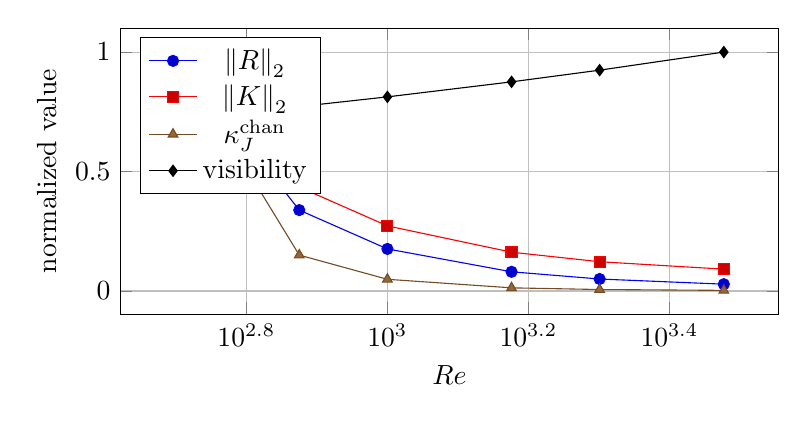
\begin{tikzpicture}
\begin{axis}[
width=0.82\linewidth,height=0.43\linewidth,
xlabel={$Re$},ylabel={normalized value},legend pos=north west,grid=both,
xmode=log,log basis x=10]
\addplot+[mark=*] coordinates {(500,1) (750,0.338546) (1000,0.175991) (1500,0.0802615) (2000,0.050054) (3000,0.028485)};
\addlegendentry{$\norm{R}_2$}
\addplot+[mark=square*] coordinates {(500,1) (750,0.434966) (1000,0.272395) (1500,0.16233) (2000,0.122411) (3000,0.0913429)};
\addlegendentry{$\norm{K}_2$}
\addplot+[mark=triangle*] coordinates {(500,1) (750,0.15025) (1000,0.0488658) (1500,0.0131074) (2000,0.00610103) (3000,0.00253164)};
\addlegendentry{$\kappa_J^{\rm chan}$}
\addplot+[mark=diamond*] coordinates {(500,0.719962) (750,0.771884) (1000,0.812419) (1500,0.875263) (2000,0.924216) (3000,1)};
\addlegendentry{visibility}
\end{axis}
\end{tikzpicture}
\caption{Integrated OS/SQ low-frequency stress-test diagnostics. Each curve is normalized by its own maximum over the displayed Reynolds numbers. The figure is not a Reynolds-number scaling claim; it shows that composite wall-to-wall response, visibility, and the transported hidden inverse-channel condition number encode different information.}
\label{fig:orr-sommerfeld-re}
\end{figure}

This benchmark should be read as a diagnostic stress test, not as the sole
validation of the theorem. It demonstrates that the theorem's quantities can be
computed in a classical nonnormal PDE discretization and that the Wedin
denominator must be taken from $\Sh$, not from the inverse resolvent $R$.


\section{Conclusion}
The channel-conditioned bound therefore provides the missing perturbation theorem for hidden Schur-complement resolvents.
The isolated-cluster assumption is essential: the results do not address embedded essential spectrum, nonclosed range, or channels without a separating singular-value gap.

The central object of this paper is the perturbation-stable restricted inverse channel transported by singular subspaces. Classical perturbation theory controls the rotation of singular subspaces; this paper bounds the inverse operator transported by those subspaces.

The independent-variation theorem shows that scalar resolvent gain and channel conditioning can separate even in finite dimensions.

The exact restricted inverse bound (Theorem~\ref{thm:channel-conditioned-stability}) explicitly separates the linear subspace-transport contribution, exactly $\kappa_J^{\rm chan} \|R\|_2 e / \| \mathcal{G}_J \|_2$, from the nonasymptotic second-order cross terms. Proposition~\ref{prop:structural-necessity} proves this bilinear gap-gain product is structurally unavoidable. 

The Orr--Sommerfeld/Squire application illustrates the physical relevance of this distinction. Modern resolvent-analysis practice likewise emphasizes the forcing-response operator, energy norm, and singular modes as implementation-level choices rather than merely scalar gains \cite{RolandiRibeiroYehTaira2024}. In the stated collocation benchmark, the full hidden resolvent, the wall-to-wall composite map, and the channel condition diagnostic report different numerical behavior. Thus the transported hidden inverse channel can be more fragile or differently aligned than a scalar input-output summary suggests, and that fragility is experimentally relevant only after diagnostic feasibility margins are declared.

\appendix
\section{Reproducibility script for tables and plots}\label{app:reproducibility}
The following Python script is the reference implementation for the Chebyshev spectral collocation of the Orr--Sommerfeld/Squire operator in Section~\ref{sec:orr-sommerfeld} and the control surrogate in Section~\ref{sec:numerics}. It uses a Chu--Kinney kinetic energy metric approximation and generates the diagnostic quantities reported in Table~\ref{tab:orr-sommerfeld-re}. Numerical values may vary slightly across BLAS/LAPACK implementations, but no table entry is analytically imposed by the manuscript text. 


\paragraph{Audit notes for the appendix implementation.}
The implementation follows the inverse-map convention used in the paper. For
$R:\calU\to\calV$, the right singular vector is the residual direction and the
left singular vector is the hidden displacement direction. Since
\texttt{scipy.linalg.svd(R)} returns \texttt{U, s, Vh}, the first row
\texttt{Vh[0,:]} is already the adjoint residual direction $u_1^*$, while
\texttt{U[:,0]} is the hidden direction $v_1$. Consequently the access and
visibility factors are computed as
\begin{equation}
    \|u_1^*M\|_2
    \quad\hbox{and}\quad
    \|Tv_1\|_2,
\end{equation}
implemented below as \texttt{V\_svd[0,:] @ M} and
\texttt{T @ U\_svd[:,0]}, respectively. This avoids the common NumPy error of
applying \texttt{.conj().T} to a one-dimensional array, where \texttt{.T} does
not form a column vector.

The appendix also follows the manuscript's ambient/restricted notation:
$\mathcal G_J=P_{V,J}\Sh^{-1}P_{U,J}$ is the ambient representative, whereas
$G_J=\mathcal G_J|_{\calU_J}$ is the physical restricted channel. The OS/SQ
benchmark is reported as a raw reference-script diagnostic for the stated
collocation, metric, frequency grid, and wall maps. The OS/SQ routine scans
frequencies from $0.05$ to $2.0$ and reports the maximizer of the channel
condition number on that grid. Finally, the gauge transformation discussed in
the text is a right-coordinate gauge, not a similarity transformation of $\Sh$.


The manuscript tables should be regenerated from this script after any change to numerical parameters.

\begin{verbatim}
import numpy as np
from scipy.linalg import eig, inv, svd, block_diag

def cheb(N):
    """Standard Chebyshev differentiation matrix."""
    if N == 0: return 0, 1
    x = np.cos(np.pi * np.arange(N+1) / N)
    c = np.array([2] + [1]*(N-1) + [2]) * (-1)**np.arange(N+1)
    X = np.tile(x, (N+1, 1))
    dX = X - X.T
    D = (c[:, None] / c[None, :]) / (dX + np.eye(N+1))
    D = D - np.diag(np.sum(D, axis=1))
    return D, x

def os_squire_benchmark(Re_list=[500, 750, 1000, 1500, 2000, 3000]):
    """Frequency-scanned OS/SQ stress test with theorem-consistent Wedin gap."""
    N = 24
    alpha, beta = 1.0, 1.0
    k2 = alpha**2 + beta**2
    omega_grid = np.linspace(0.05, 2.0, 16)

    D, x = cheb(N)
    y = x[1:N]
    D2full = D @ D
    D4full = D2full @ D2full
    D2 = D2full[1:N, 1:N]
    D4 = D4full[1:N, 1:N]
    I = np.eye(N-1)

    U = np.diag(1 - y**2)
    Uy = np.diag(-2 * y)
    Delta = D2 - k2 * I
    invDelta = inv(Delta)

    # Chu-Kinney-type kinetic energy metric approximation.
    W_OS = -Delta / k2
    W_SQ = I / k2
    W = block_diag(W_OS, W_SQ)
    W = 0.5 * (W + W.conj().T)
    ew, Qw = np.linalg.eigh(W)
    ew = np.maximum(ew, 1e-12)
    W_half = Qw @ np.diag(np.sqrt(ew)) @ Qw.conj().T
    W_invhalf = Qw @ np.diag(1 / np.sqrt(ew)) @ Qw.conj().T

    m = 2 * (N-1)
    M = np.zeros((m, 1), dtype=complex)
    T = np.zeros((1, m), dtype=complex)
    M[0, 0] = 1.0
    T[0, 0] = 1.0

    print("Re omega* ||R||_2 ||K||_2 omega_Sh kappa Access Visibility")
    for Re in Re_list:
        LOS = invDelta @ (
            -1j * alpha * (U @ Delta - (-2 * I))
            + (D4 - 2*k2*D2 + (k2**2)*I) / Re
        )
        LSQ = -1j * alpha * U + (D2 - k2 * I) / Re
        C = -1j * beta * Uy
        L = np.block([[LOS, np.zeros((N-1, N-1), dtype=complex)], [C, LSQ]])

        best = None
        for omega_f in omega_grid:
            Sh_raw = 1j * omega_f * np.eye(m) - L
            R_raw = inv(Sh_raw)

            R = W_half @ R_raw @ W_invhalf
            Sh_w = W_half @ Sh_raw @ W_invhalf

            U_svd, sR, Vh = svd(R, full_matrices=False)
            sh_svals = np.sort(svd(Sh_w, compute_uv=False))

            gain = sR[0]
            omega_j = max(sh_svals[1] - sh_svals[0], np.finfo(float).eps)
            kappa = gain / omega_j
            K_mat = T @ R @ M

            # Vh[0, :] is the adjoint residual direction u_1^*.
            access = np.linalg.norm(Vh[0, :] @ M, 2)
            # U_svd[:, 0] is the hidden displacement direction v_1.
            visibility = np.linalg.norm(T @ U_svd[:, 0], 2)

            row = (Re, omega_f, gain, np.linalg.norm(K_mat, 2),
                   omega_j, kappa, access, visibility)
            if best is None or row[5] > best[5]:
                best = row

        print(
            f"{best[0]:4d} {best[1]:6.3f} {best[2]:.6e} {best[3]:.6e} "
            f"{best[4]:.6e} {best[5]:.6e} {best[6]:.6e} {best[7]:.6e}"
        )


def chain_matrices(n=40, beta=0.0, omega=0.8):
    """Forty-state control surrogate from Section 8."""
    e = np.ones(n)
    D2 = np.diag(-2*e) + np.diag(e[:-1], 1) + np.diag(e[:-1], -1)
    D1 = np.diag(e[:-1], 1) - np.diag(e[:-1], -1)
    N_mat  = np.triu(np.ones((n, n)), 1)
    A  = 0.004*D2 - 0.04*np.eye(n) + (0.15/n)*D1 + (beta/n)*N_mat
    S  = 1j*omega*np.eye(n) - A
    M = np.zeros((n, 3)); M[[5, 17, 31], [0, 1, 2]] = 1.0
    T = np.zeros((3, n)); T[[0, 1, 2], [9, 24, 37]] = 1.0
    return S, M, T


def chain_matrices_benchmark(beta_list=[0, 2, 4, 6, 8, 10]):
    """Evaluates the 40-state surrogate to reproduce Table 2."""
    print("\nbeta sigma_min gain omega_J kappa access vis K_gain")
    # Values below 1e-13 are displayed in the manuscript table as <10^{-13}.
    for beta in beta_list:
        S, M, T = chain_matrices(n=40, beta=beta, omega=0.8)
        R = inv(S)
        U_svd, sR, Vh = svd(R, full_matrices=False)
        gain = sR[0]

        # Explicitly compute the Wedin gap from Sh, not from R.
        sS = np.sort(svd(S, compute_uv=False))
        sigma_min = sS[0]
        omega_j = sS[1] - sS[0]
        kappa = gain / omega_j

        K_mat = T @ R @ M
        k_gain = np.linalg.norm(K_mat, 2)

        # Vh[0, :] is u_1^* and U_svd[:, 0] is v_1.
        access = np.linalg.norm(Vh[0, :] @ M, 2)
        vis = np.linalg.norm(T @ U_svd[:, 0], 2)

        k_str = "<10^{-13}" if k_gain < 1e-13 else f"{k_gain:.4f}"
        print(
            f"{beta:2d} {sigma_min:.4f} {gain:.4f} {omega_j:.4f} "
            f"{kappa:.4f} {access:.4f} {vis:.4f} {k_str}"
        )


if __name__ == '__main__':
    os_squire_benchmark()
    chain_matrices_benchmark()
\end{verbatim}


\section*{Acknowledgements}
The authors acknowledge the financial support of \textless anonymous for review\textgreater{} and thank participants at \textless anonymous for review\textgreater{}, especially \textless anonymous for review\textgreater{}, for constructive comments on earlier drafts. The mathematical formulations and principal analyses are the original work of the authors. Selected computational tools, including WolframAlpha, SageMath, etc., were used for verification and graphical support. Large language model--based tools contributed to proofreading, formatting, and editorial refinement during the final preparation of the manuscript.

\begin{thebibliography}{99}

\bibitem{GohbergGoldbergKaashoek1990}
I. Gohberg, S. Goldberg, and M. A. Kaashoek, \emph{Classes of Linear Operators, Vol. I}, Birkh\"auser, Basel, 1990.

\bibitem{Bhatia1997}
R. Bhatia, \emph{Matrix Analysis}, Springer, New York, 1997.

\bibitem{DavisKahan1970}
C. Davis and W. M. Kahan, The rotation of eigenvectors by a perturbation. III, \emph{SIAM J. Numer. Anal.}, 7 (1970), pp. 1--46.

\bibitem{Kato1995}
T. Kato, \emph{Perturbation Theory for Linear Operators}, Springer, Berlin, 1995.

\bibitem{StewartSun1990}
G. W. Stewart and J.-G. Sun, \emph{Matrix Perturbation Theory}, Academic Press, Boston, 1990.

\bibitem{Wedin1972}
P.-A. Wedin, Perturbation bounds in connection with singular value decomposition, \emph{BIT}, 12 (1972), pp. 99--111.

\bibitem{SchmidHenningson2001}
P. J. Schmid and D. S. Henningson, \emph{Stability and Transition in Shear Flows}, Springer, New York, 2001.

\bibitem{ZhouDoyleGlover1996}
K. Zhou, J. C. Doyle, and K. Glover, \emph{Robust and Optimal Control}, Prentice Hall, Upper Saddle River, 1996.

\bibitem{BennerGugercinWillcox2015}
P. Benner, S. Gugercin, and K. Willcox, A survey of projection-based model reduction methods for parametric dynamical systems, \emph{SIAM Rev.}, 57 (2015), pp. 483--531.

\bibitem{ReddySchmidHenningson1993}
S. C. Reddy, P. J. Schmid, and D. S. Henningson, Pseudospectra of the Orr--Sommerfeld operator, \emph{SIAM J. Appl. Math.}, 53 (1993), pp. 15--47.

\bibitem{JovanovicBamieh2005}
M. R. Jovanovi\'c and B. Bamieh, Componentwise energy amplification in channel flows, \emph{J. Fluid Mech.}, 534 (2005), pp. 145--183.

\bibitem{McKeonSharma2010}
B. J. McKeon and A. S. Sharma, A critical-layer framework for turbulent pipe flow, \emph{J. Fluid Mech.}, 658 (2010), pp. 336--382.

\bibitem{TrefethenEmbree2005}
L. N. Trefethen and M. Embree, \emph{Spectra and Pseudospectra: The Behavior of Nonnormal Matrices and Operators}, Princeton University Press, Princeton, 2005.


\bibitem{RolandiRibeiroYehTaira2024}
L. V. Rolandi, J. H. M. Ribeiro, C.-A. Yeh, and K. Taira, An invitation to resolvent analysis, arXiv:2404.11789, 2024.

\bibitem{ZulfiqarXiaoSongSreeram2025}
U. Zulfiqar, Z.-H. Xiao, Q.-Y. Song, and V. Sreeram, Balanced truncation via tangential interpolation, arXiv:2409.13358v2, 2025.

\bibitem{StraesserWorthmannMezicBerberichSchallerAllgower2026}
R. Str\"asser, K. Worthmann, I. Mezi\'c, J. Berberich, M. Schaller, and F. Allg\"ower, An overview of Koopman-based control: From error bounds to closed-loop guarantees, \emph{Annual Reviews in Control}, 61 (2026), 101035.

\end{thebibliography}

\clearpage
\section*{Summary of Notation}
Table~\ref{tab:summary-notation} summarizes the principal notation used throughout the manuscript. It is placed at the end for reference while reading.

{\small
\renewcommand{\arraystretch}{1.08}
\begin{tabularx}{\textwidth}{@{}L{0.24\textwidth}Y@{}}
\toprule
\textbf{Symbol} & \textbf{Meaning}\\
\midrule
$\calU,\calV$ & Hidden residual and hidden displacement Hilbert spaces.\\
$\Sh:\calV\to\calU$ & Hidden Schur-complement operator whose inverse defines the hidden response.\\
$R=\Sh^{-1}$ & Hidden inverse or resolvent map from residual directions to hidden displacement directions.\\
$M,T$ & Actuation and observation maps: $M$ injects external inputs into the hidden residual space, and $T$ observes hidden displacements.\\
$K=T\Sh^{-1}M$ & Measured composite input-output map.\\
$U_J,V_J$ & Left and right singular subspaces associated with an isolated singular cluster $J$ of $\Sh$.\\
$P_{U,J},P_{V,J}$ & Orthogonal projectors onto $U_J$ and $V_J$.\\
$\mathcal G_J=P_{V,J}\Sh^{-1}P_{U,J}$ & Ambient representative of the restricted hidden inverse channel.\\
$G_J=\mathcal G_J|_{\calU_J}$ & Physical restricted channel acting on the selected singular input subspace.\\
$\omega_J$ & Wedin singular-value separation between cluster $J$ and its complement.\\
$\kappa_J^{\rm chan}=\norm{\mathcal G_J}/\omega_J$ & Channel condition number: inverse-channel gain normalized by singular-subspace separation.\\
$\smin(U_J^*M)$ & Access: how well the actuators excite the selected hidden singular directions.\\
$\smin(TV_J)$ & Visibility: how well the sensors observe the selected hidden singular directions.\\
$\Sigma_J,\Sigma_\perp$ & Singular-value blocks for the selected cluster and its orthogonal complement in the normal form.\\
$\theta_{\max}(\calV_J,\widetilde{\calV}_J)$ & Largest principal-angle separation between two right singular subspaces.\\
$E,e$ & Operator perturbation and its norm, usually $e=\norm{E}$.\\
$\widetilde{\Sh},\widetilde G_J$ & Perturbed operator and perturbed restricted channel.\\
$\delta_W$ & Size of an admissible metric or weight perturbation.\\
$\omega_f$ & Frequency parameter used in the OS/SQ stress-test computations.\\
\bottomrule
\end{tabularx}}
\label{tab:summary-notation}

\end{document}
